\documentclass[a4paper,12pt]{report} % размер бумаги устанавливаем А4, шрифт 12 пунктов
\usepackage[T2A]{fontenc} % поддержка кириллицы в ЛаТеХ
\usepackage[utf8]{inputenc} % настройка кодировки
\usepackage[english,russian]{babel} % Определение языков в документе
\usepackage{amssymb,amsfonts,amsmath,mathtext,cite,enumerate,float} % подключаем нужные пакеты расширений
\usepackage{indentfirst} % делать отступ в начале параграфа
\usepackage{tabularx} % продвинутые таблицы
% \usepackage{showkeys} % раскомментировать, чтобы в документе были видны ссылки на литературу, рисунки и таблицы
\usepackage[labelsep=period]{caption} % заменить умолчальное разделение ':' на '.' в подписях к рисункам и таблицам
\usepackage[onehalfspacing]{setspace} % "умное" расстояние между строк - установить 1.5 интервала от нормального
\usepackage[final]{graphicx} % разрешить включение PostScript-графики
\graphicspath{{img/}} % Относительный путь к каталогу с рисунками

\usepackage{textcomp}
\newcommand*{\No}{\textnumero}

\makeatletter
\bibliographystyle{unstr} % Стиль библиографических ссылок БибТеХа - нумеровать в порядке упоминания в тексте
\renewcommand{\@biblabel}[1]{#1.} % Заменяем библиографию с квадратных скобок на точку в списке литературы
\makeatother

\def\labelitemi{--} % установка префикса немаркированного списка

% Настройка геометрии
\usepackage{geometry}
\geometry{left=2cm}
\geometry{right=1.5cm}
\geometry{top=1cm}
\geometry{bottom=2cm}

% настройка листинга
\usepackage{color} %% это для отображения цвета в коде
\usepackage{xcolor}
\usepackage{listings} %% собственно, это и есть пакет listings

\usepackage{hyperref}
\usepackage{multirow}
\usepackage{enumitem}

\DeclareCaptionFont{white}{\color{white}} %% это сделает текст заголовка белым
%% код ниже нарисует серую рамочку вокруг заголовка кода.
\DeclareCaptionFormat{listing}{\colorbox{gray}{\parbox{\textwidth}{#1#2#3}}}
\captionsetup[lstlisting]{format=listing,labelfont=white,textfont=white}
\lstset{ %
language=C, % выбор языка для подсветки (здесь это С)
basicstyle=\small\sffamily, % размер и начертание шрифта для подсветки кода
numbers=left, % где поставить нумерацию строк (слева\справа)
%numberstyle=\tiny, % размер шрифта для номеров строк
stepnumber=1, % размер шага между двумя номерами строк
numbersep=5pt, % как далеко отстоят номера строк от подсвечиваемого кода
backgroundcolor=\color{white}, % цвет фона подсветки - используем \usepackage{color}
showspaces=false, % показывать или нет пробелы специальными отступами
showstringspaces=false, % показывать или нет пробелы в строках
showtabs=false, % показывать или нет табуляцию в строках
frame=single, % рисовать рамку вокруг кода
tabsize=2, % размер табуляции по умолчанию равен 2 пробелам
captionpos=t, % позиция заголовка вверху [t] или внизу [b]
breaklines=true, % автоматически переносить строки (да\нет)
breakatwhitespace=false, % переносить строки только если есть пробел
escapeinside={\%*}{*)} % если нужно добавить комментарии в коде
}

% Меняем везде перечисления на цифра.цифра
\renewcommand{\theenumi}{\arabic{enumi}}
\renewcommand{\labelenumi}{\arabic{enumi}}
\renewcommand{\theenumii}{\arabic{enumii}}
\renewcommand{\labelenumii}{\arabic{enumi}.\arabic{enumii}.}
\renewcommand{\theenumiii}{\arabic{enumiii}}
\renewcommand{\labelenumiii}{\arabic{enumi}.\arabic{enumii}.\arabic{enumiii}.}

\renewcommand{\thesection}{\arabic{section}.}
% \renewcommand{\thesubsection}{\arabic{section}.\arabic{subsection}.}
\renewcommand{\thesubsection}{\arabic{subsection}.}
% \renewcommand{\thesubsubsection}{\arabic{section}.\arabic{subsection}.\arabic{subsubsection}.}
\renewcommand{\thesubsubsection}{\arabic{subsection}.\arabic{subsubsection}.}

\newtheorem{theorem}{Theorem}
\usepackage{subcaption}

\begin{document}
\def\figurename{Figure} % префикс к рисунками
\def\tablename{Table}
\newpage
\begin{titlepage}

\begin{center}\large{
    FEDERAL STATE AUTONOMOUS EDUCATIONAL INSTITUTION \\
    OF HIGHER EDUCATION \\*
    ITMO UNIVERSITY \\*
}\end{center}

\vspace{12em}

\begin{center}\large{
    Report \\
    on the practical task No. 7 \\
    <<Algorithms on graphs.
    Tools for network analysis>>
}\end{center}

\vspace{8.5em}

\flushright{Performed by}
\flushright{Sultan Zhumabaev}
\flushright{J4133c}
\vspace{1.5em}
\flushright{Accepted by}
\flushright{Dr Petr Chunaev}

\vspace{\fill}

\begin{center}
    St. Petersburg \\
    2020
\end{center}

\end{titlepage}

% \tableofcontents
\newpage
\subsection{Goal}\label{subsec:goal}

The use of the network analysis software Gephi.

\subsection{Formulation of the problem}\label{subsec:formulation-of-the-problem}

\begin{enumerate}
    \item Download and install Gephi from \url{https://gephi.org/}.
    \item Choose a network dataset from \url{https://snap.stanford.edu/data/} with number of nodes at most 10,000.
    You are free to choose the network nature and type (un/weighted, un/directed).
    \item Change the format of the dataset for that accepted by Gephi (.csv, .xls, .edges, etc.), if necessary.
    \item Upload and process the dataset in Gephi. Check if the parameters of import and data are correct.
    \item Obtain a graph layout of two different types.
    \item Calculate available network measures in Statistics provided by Gephi.
    \item Analyze the results for the network chosen.
\end{enumerate}

While performing the work, screenshot the main steps you are doing and insert in the report.

\subsection{Brief theoretical part}\label{subsec:brief-theoretical-part}

\paragraph{Gephi.}

\textit{Gephi} is an interactive visualization and exploration platform for all kinds of networks and complex systems, dynamic and hierarchical graphs.

\paragraph{Dataset information.}

This is who-trusts-whom network of people who trade using Bitcoin on a platform called Bitcoin Alpha.
Since Bitcoin users are anonymous, there is a need to maintain a record of users' reputation to prevent transactions with fraudulent and risky users.
Members of Bitcoin Alpha rate other members in a scale of -10 (total distrust) to +10 (total trust) in steps of 1.
This is the first explicit weighted signed directed network available for research.

\paragraph{Dataset statistics:}
\begin{itemize}
    \item nodes: 3,783;
    \item edges: 24,186;
    \item range of edge weight: -10 to +10;
    \item percentage of positive edges: 93\%.
\end{itemize}

\paragraph{Main characteristics.}
Characteristics of degrees of vertices of an unweighted graph:
\begin{itemize}
    \item $d(v), \text{degree} v$, - number of incoming and outgoing edges of vertex $v$;
    \item $d_{in}(v), \text{half-step of approach} v$, - the number of incoming edges of vertex $v$;
    \item $\bar{d} = \frac{1}{\lvert V \rvert}\sum_{v \in V}{d(v)}$ - the average degree of vertices.
\end{itemize}

For a weighted graph, similar values can be entered, with the only difference that they do not take into account the number of edges, but the sum of the weights on the edges.

Graph characteristics in terms of distances:
\begin{itemize}
    \item $dist(v, u)$ - the distance between $v$ and $u$;
    \item \textit{eccentricity} $\epsilon(v) = \max_{u \in V}dist(v, u)$ - the greatest distance between $v$ and other vertexes;
    \item \textit{radius} $r = \min_{v \in V}\epsilon(v)$ - the minimum eccentricity across all vertices;
    \item \textit{diameter} $D = \max_{v \in V}\epsilon(v)$ - the highest eccentricity of all the nodes;
    \item \textit{average path length} $l = \frac{1}{\lvert V \rvert(\lvert V \rvert - 1)}\sum_{v \neq u}dist(v, u)$.
\end{itemize}

\textit{The density} $\rho$ of a graph is the quotient of $\lvert E \rvert$ and the number of possible edges with the same $\lvert V \rvert$, i.e.\ the number of edges in a complete graph with $\lvert V \rvert$ vertices:
\begin{equation*}
    \rho = \frac{2\lvert E \rvert}{\lvert V \rvert(\lvert V \rvert - 1)}.
\end{equation*}

\paragraph{Main steps.}
Review and describe the main steps when working with the Gephi tool:
\begin{enumerate}
    \item Select the file with the graph in the start window (Figure~\ref{ris:start}).
        \begin{figure}[H]
        \center
        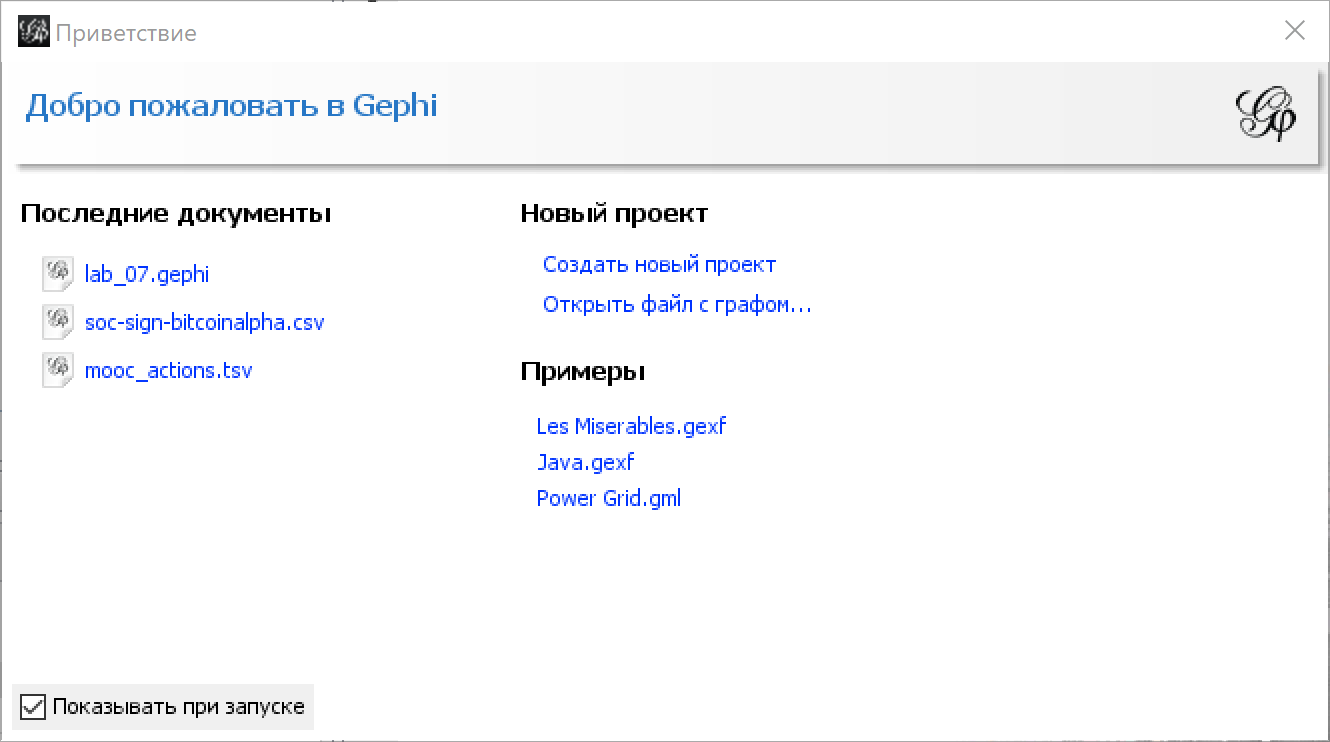
\includegraphics[width=\textwidth]{img/start.png}
        \caption{Start window of the Gephi}
        \label{ris:start}
        \end{figure}
    \item Configuring data import (Figure~\ref{ris:import_settings}).
        \begin{figure}[H]
            \centering
            \begin{subfigure}{.49\textwidth}
                \centering
                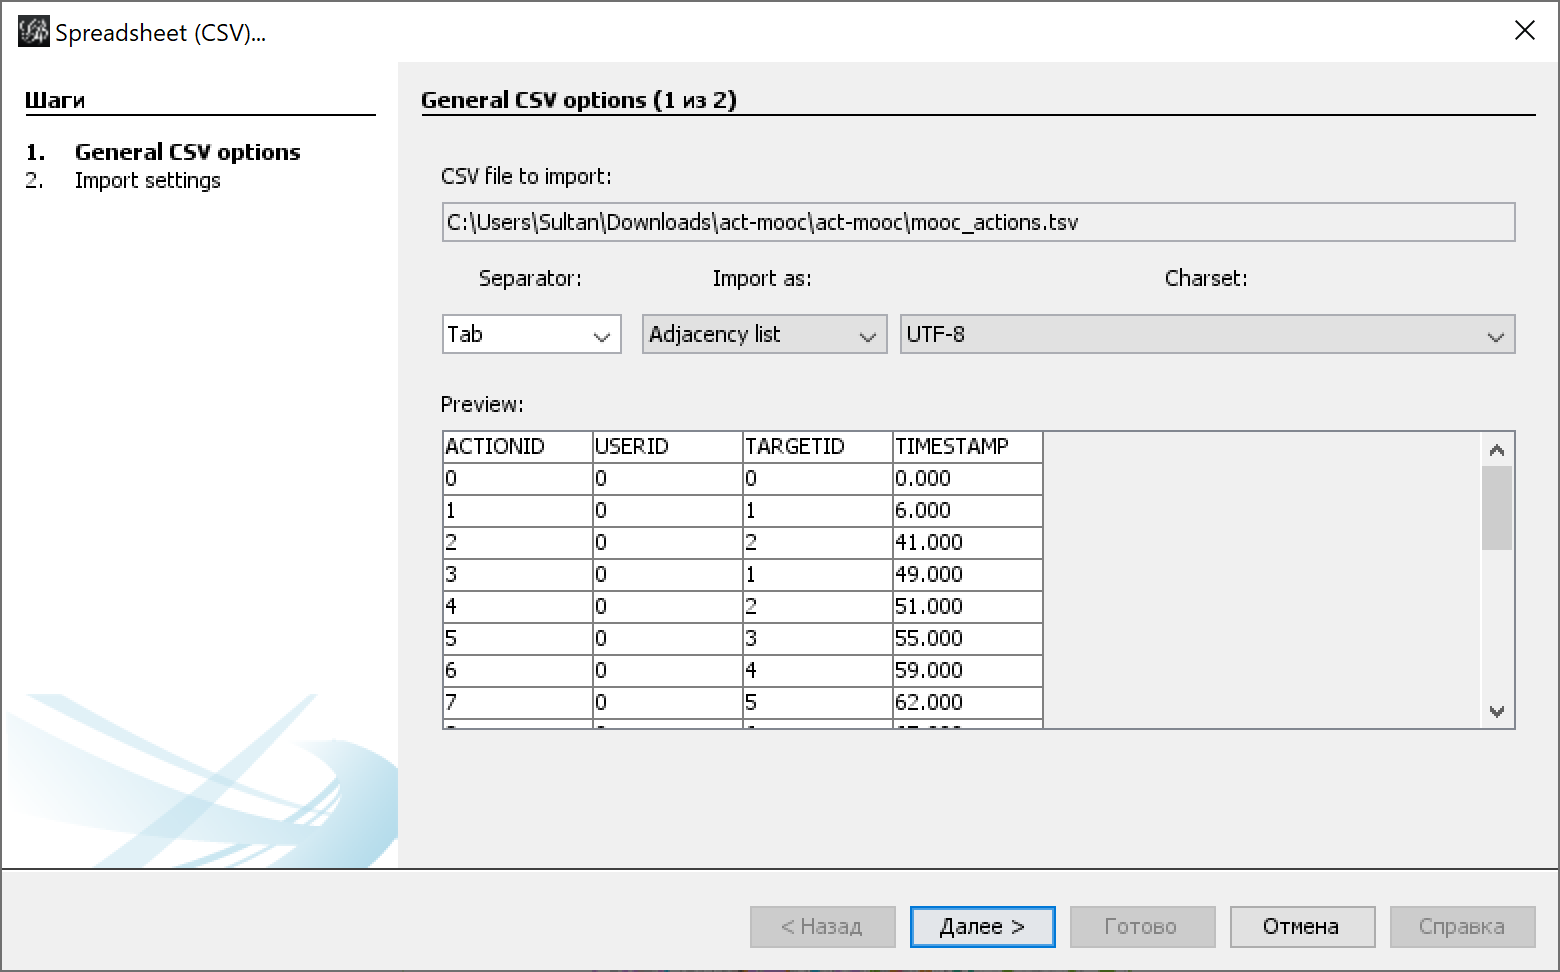
\includegraphics[width=\textwidth]{img/csv_options.png}
                \caption{General CSV options}
            \end{subfigure}
            \begin{subfigure}{.49\textwidth}
                \centering
                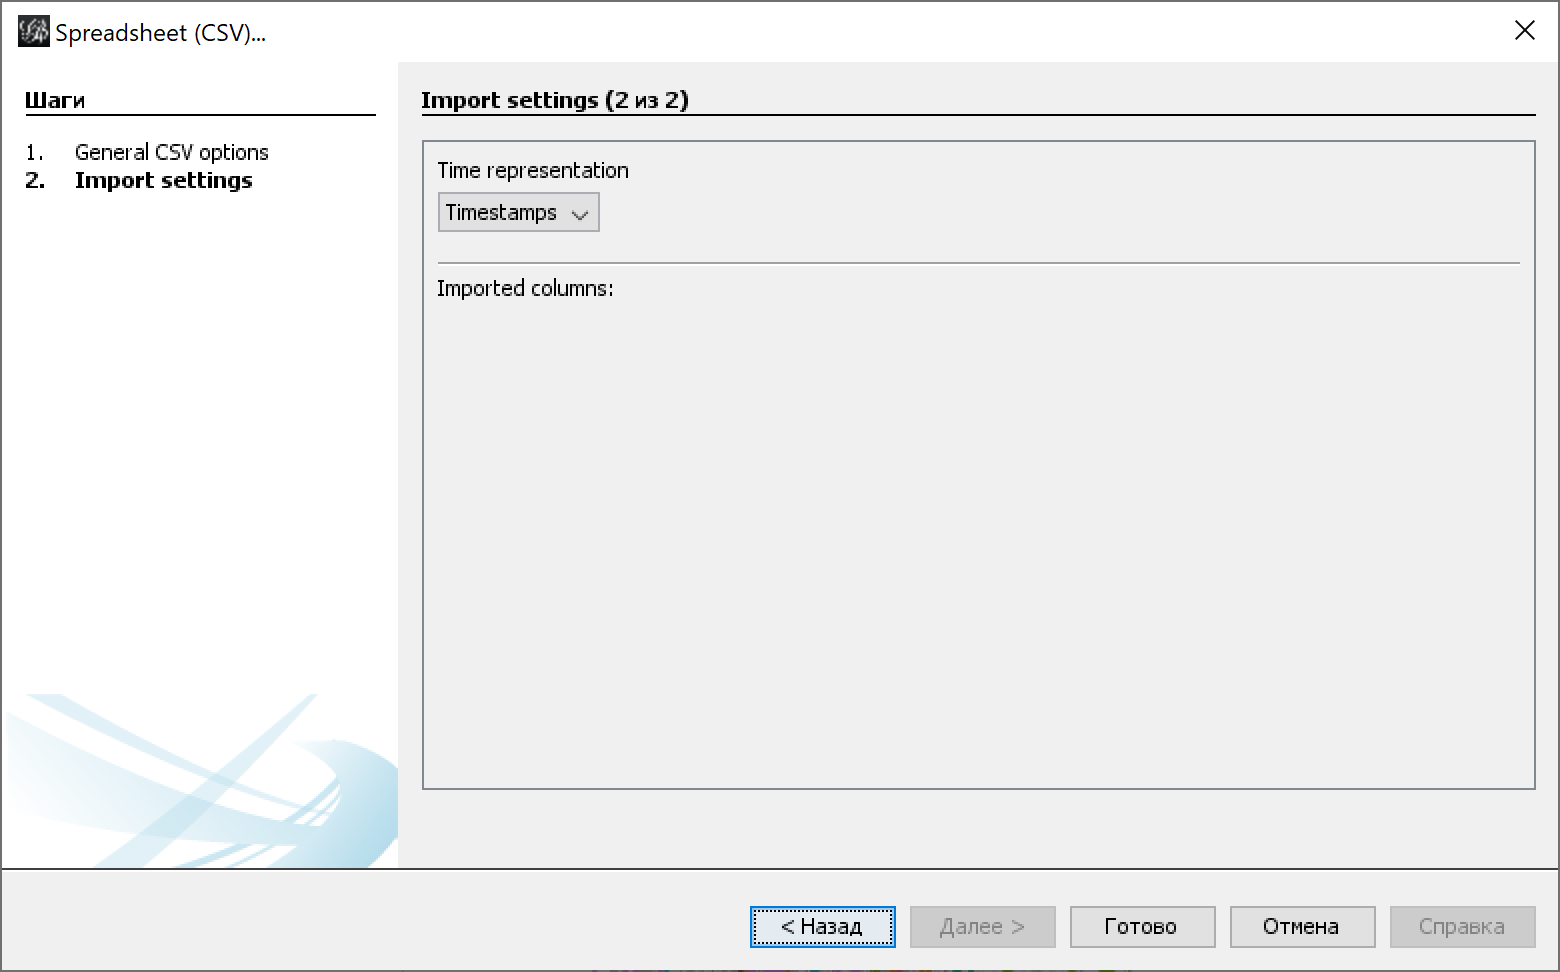
\includegraphics[width=\textwidth]{img/import.png}
                \caption{Import settings}
            \end{subfigure}
            \caption{Spreadsheet (CSV)}
            \label{ris:import_settings}
        \end{figure}
    \item Choosing different graph layouts (Figure~\ref{ris:layouts}).
        \begin{figure}[H]
            \centering
            \begin{subfigure}{\textwidth}
                \centering
                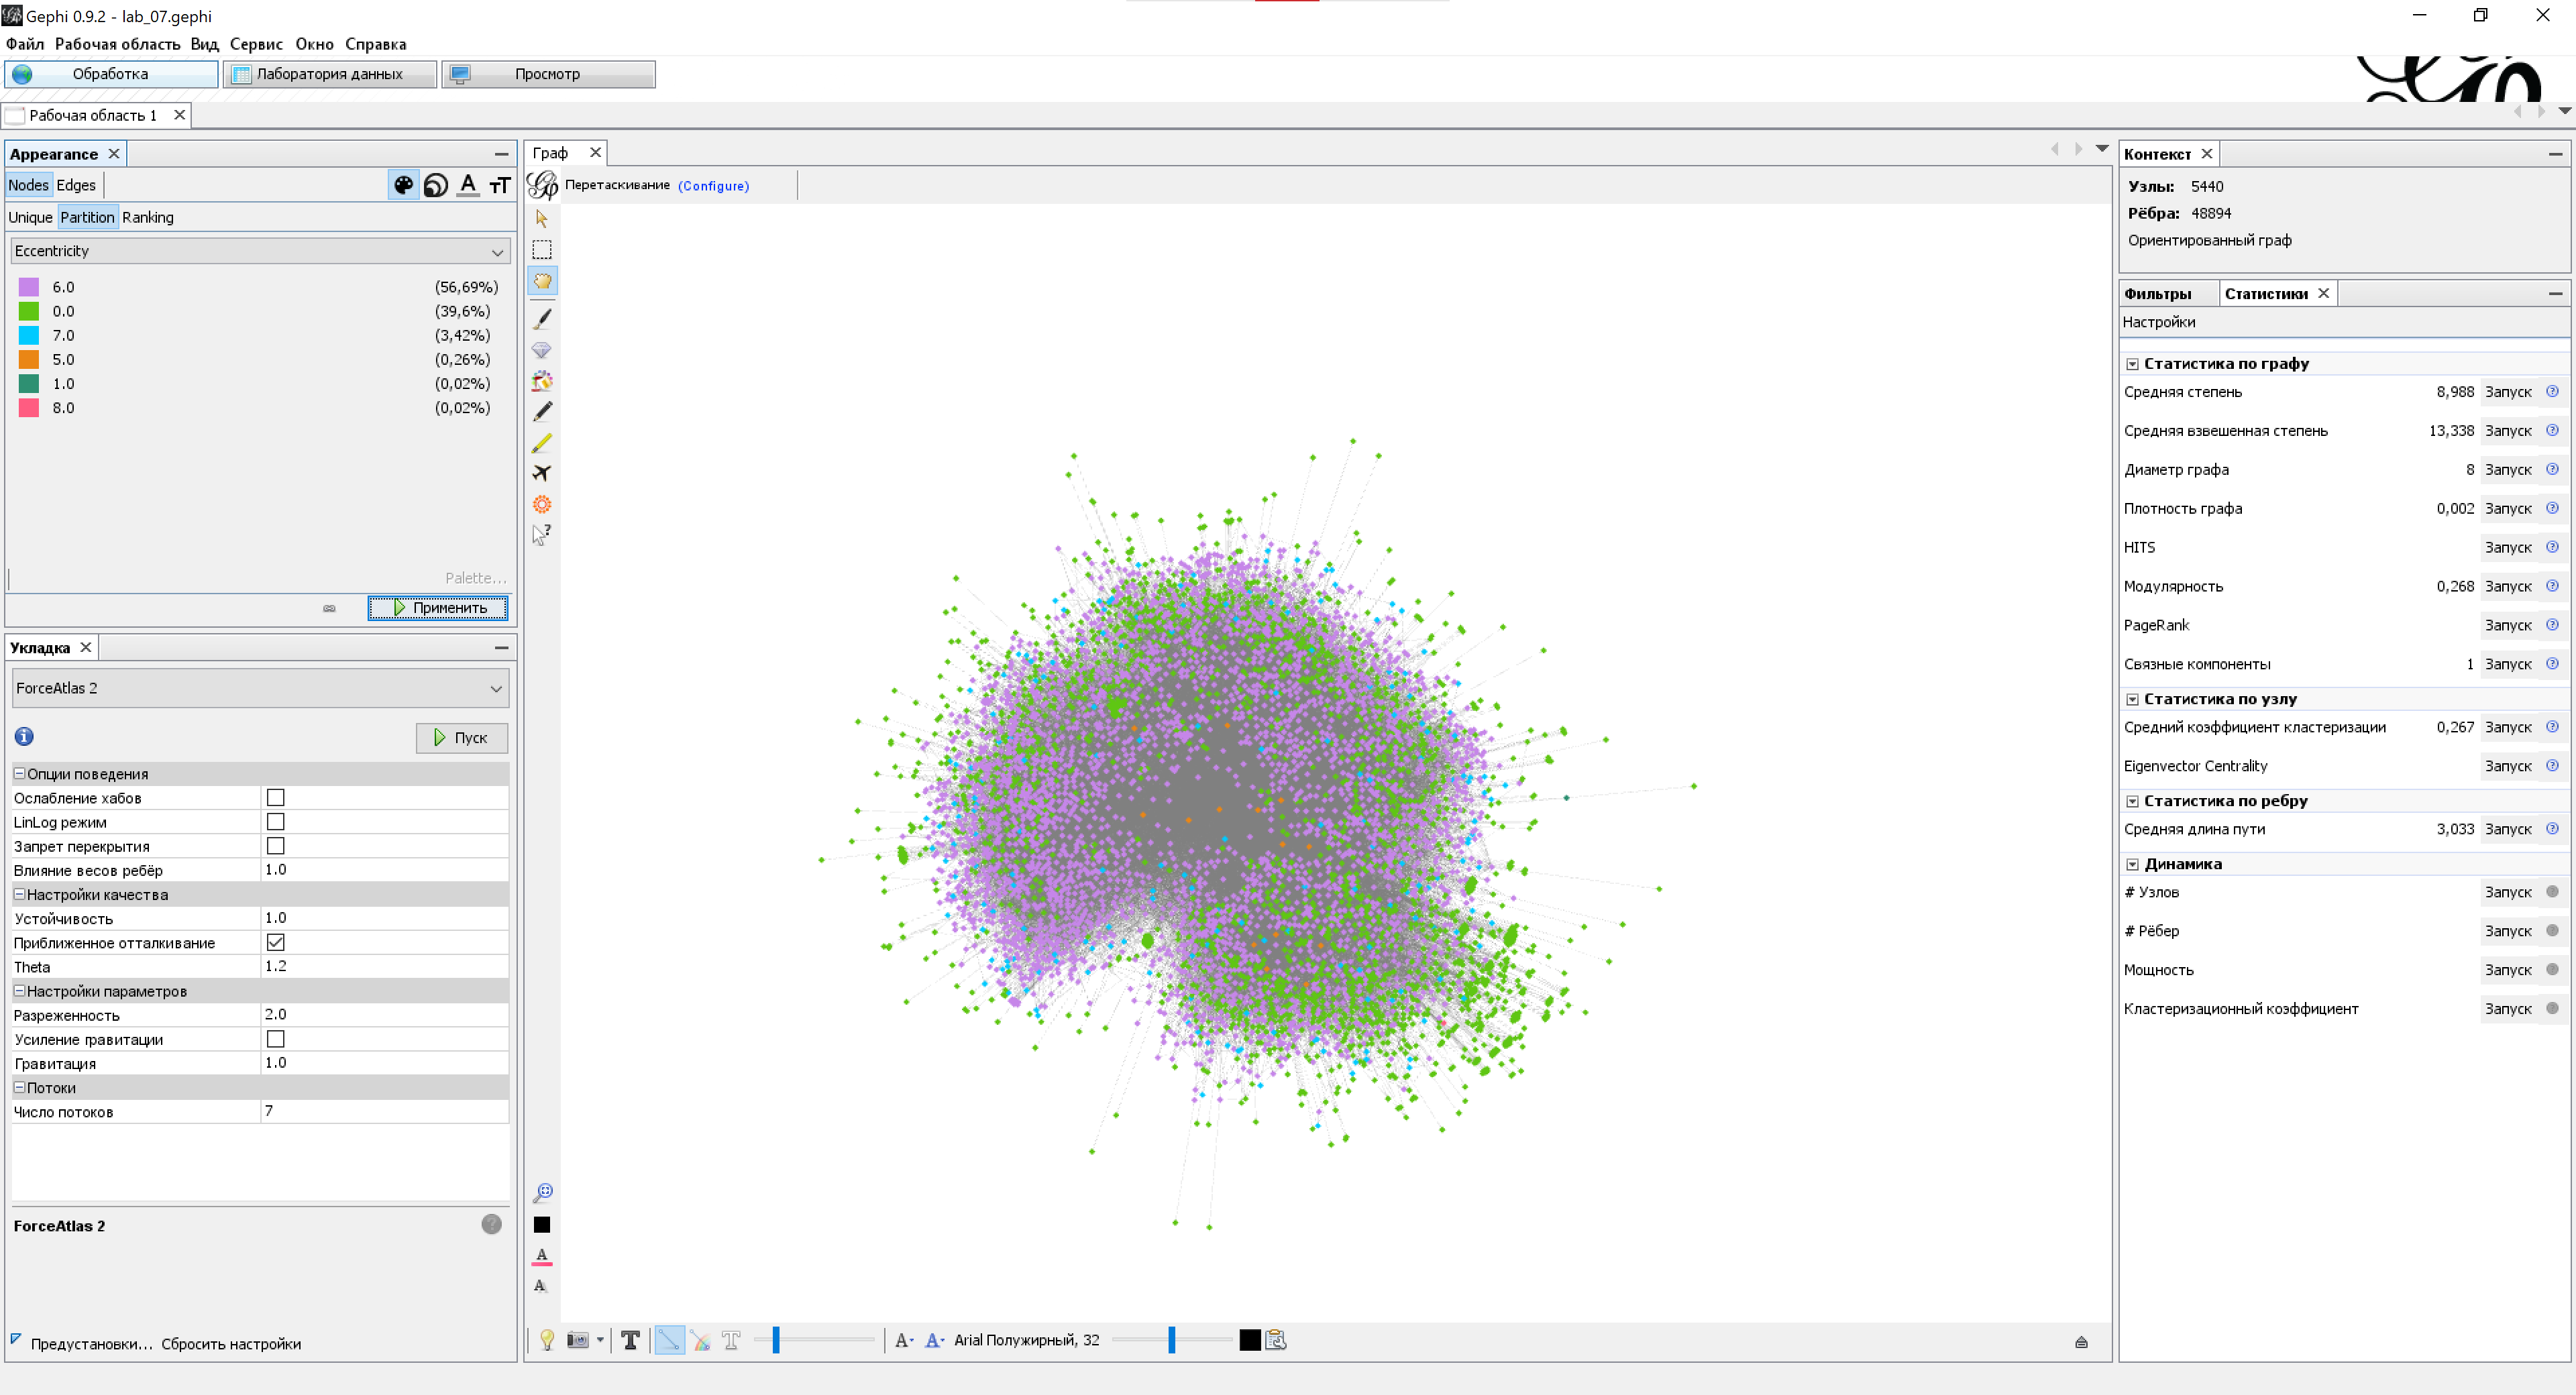
\includegraphics[width=\textwidth]{img/layout_forceatlas_2.png}
                \caption{ForceAtlas 2 layout}
            \end{subfigure}
            \begin{subfigure}{\textwidth}
                \centering
                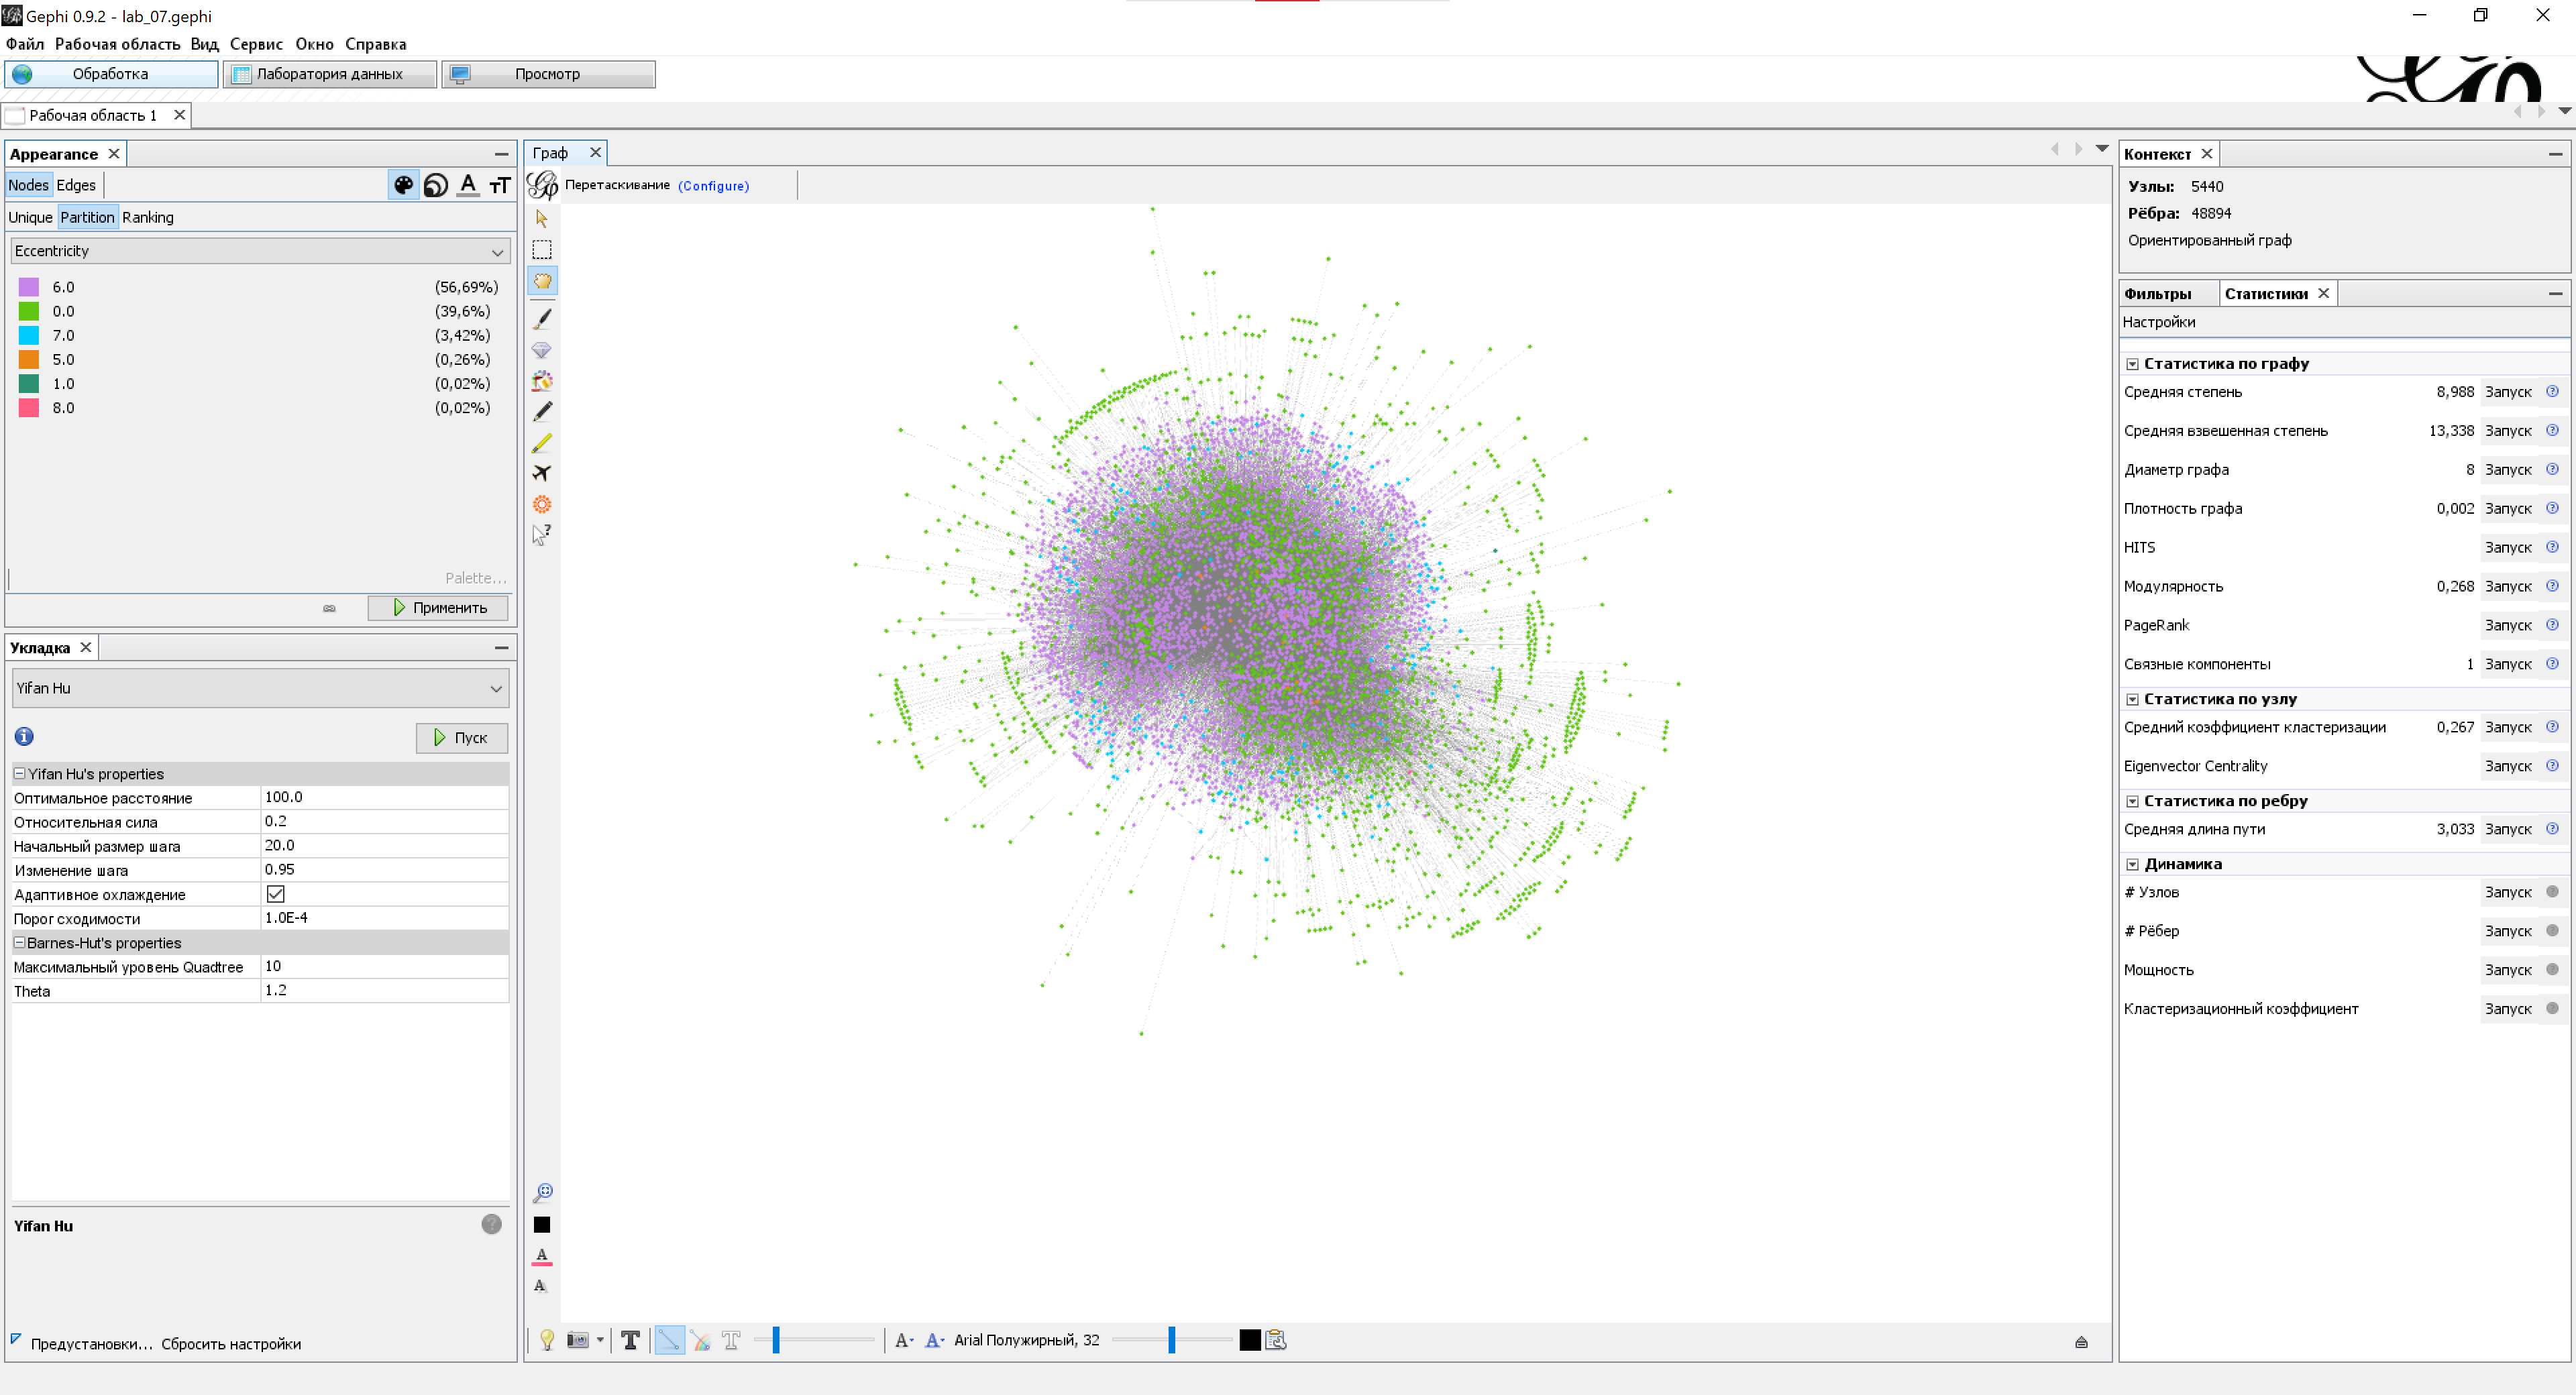
\includegraphics[width=\textwidth]{img/layout_yifanhu.png}
                \caption{Yifan Hu layout}
            \end{subfigure}
            \caption{Example of how Gephi works for the network}
            \label{ris:layouts}
        \end{figure}
\end{enumerate}

\subsection{Results}\label{subsec:results}

\textbf{Network overview:}
\begin{enumerate}
    \item \textit{Average Degree} - 8.988.
    \item \textit{Avg.\ Weighted Degree} - 13.338.
    \item \textit{Network Diameter} - 8.
    \item \textit{Graph Density} - 0.002 (sparse graph).
    \item \textit{HITS} is metric determines two values for a page (Figure~\ref{ris:hits}): its authority, which estimates the value of the content of the page, and its hub value, which estimates the value of its links to other pages.
        \begin{figure}[H]
            \centering
            \begin{subfigure}{0.49\textwidth}
                \centering
                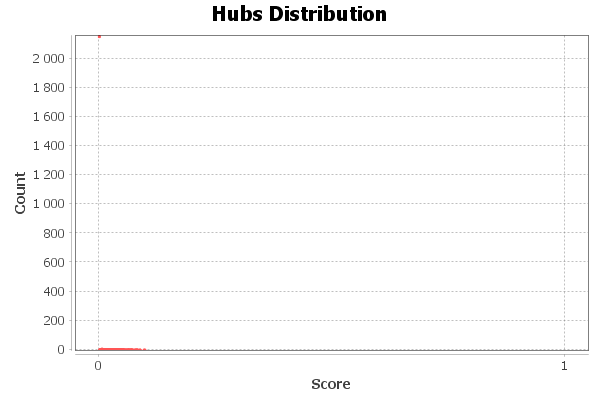
\includegraphics[width=\textwidth]{img/hits_hubs.png}
                \caption{Hubs distribution}
            \end{subfigure}
            \begin{subfigure}{0.49\textwidth}
                \centering
                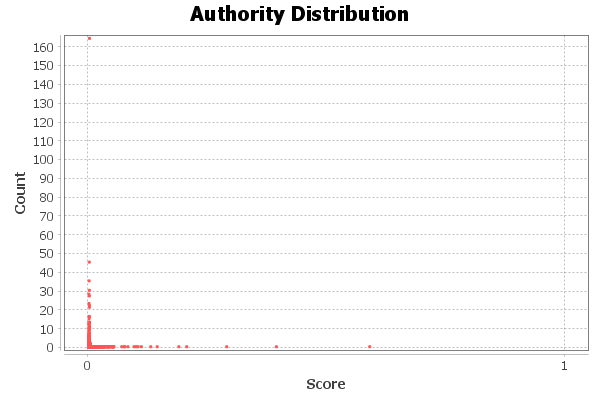
\includegraphics[width=\textwidth]{img/hits_authority.png}
                \caption{Authority distribution}
            \end{subfigure}
            \caption{HITS Metric Report}
            \label{ris:hits}
        \end{figure}
    \item \textit{Modularity} is the strength of division of a network into modules - 0.268.
    \item \textit{PageRank} is used to measure importance of a node, calculating number of incoming edges of the said node (Figure~\ref{ris:pagerank}).
        \begin{figure}[H]
        \center
        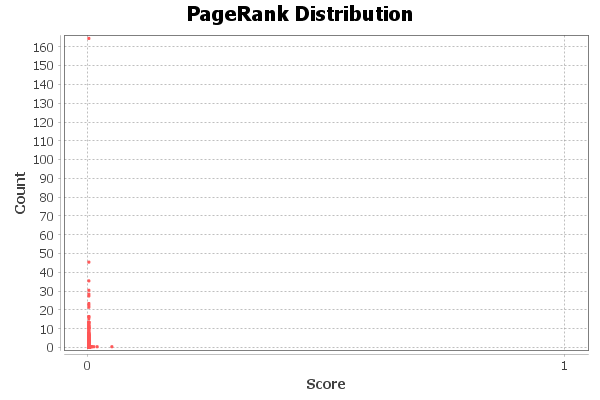
\includegraphics[width=\textwidth]{img/pagerank.png}
        \caption{PageRank distribution}
        \label{ris:pagerank}
        \end{figure}
    \item \textit{Connected Components} - 1.
\end{enumerate}

\textbf{Node overview:}
\begin{enumerate}
    \item \textit{Avg.\ Clustering Coefficient} - 0.267.
    \item \textit{Eigenvector Centrality} is used to measure the level of influence of a node within a network (Figure~\ref{ris:eigenvector}).
        \begin{figure}[H]
        \center
        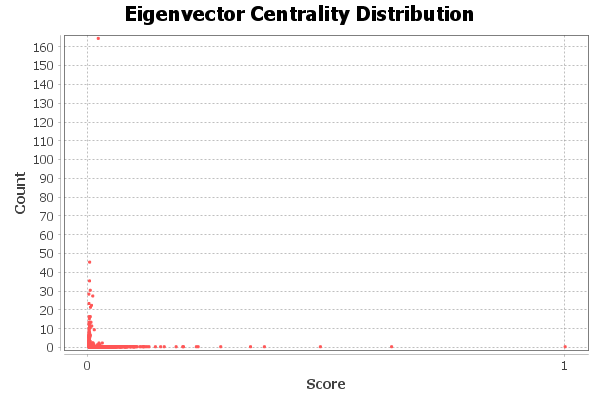
\includegraphics[width=\textwidth]{img/eigenvector.png}
        \caption{Eigenvector centrality distribution}
        \label{ris:eigenvector}
        \end{figure}
\end{enumerate}

\textbf{Edge overview:}
\begin{enumerate}
    \item \textit{Avg.\ Path Length} - 3.003.
\end{enumerate}

\subsection{Conclusion}\label{subsec:conclusion}

This task uses the Gephi network analysis tool.
The main characteristics of the network are analyzed.

\subsection{Appendix}\label{subsec:appendix}

Source dataset: \url{https://snap.stanford.edu/data/soc-sign-bitcoin-alpha.html}.

\end{document}
